% Options for packages loaded elsewhere
\PassOptionsToPackage{unicode}{hyperref}
\PassOptionsToPackage{hyphens}{url}
%
\documentclass[
]{book}
\usepackage{amsmath,amssymb}
\usepackage{lmodern}
\usepackage{iftex}
\ifPDFTeX
  \usepackage[T1]{fontenc}
  \usepackage[utf8]{inputenc}
  \usepackage{textcomp} % provide euro and other symbols
\else % if luatex or xetex
  \usepackage{unicode-math}
  \defaultfontfeatures{Scale=MatchLowercase}
  \defaultfontfeatures[\rmfamily]{Ligatures=TeX,Scale=1}
\fi
% Use upquote if available, for straight quotes in verbatim environments
\IfFileExists{upquote.sty}{\usepackage{upquote}}{}
\IfFileExists{microtype.sty}{% use microtype if available
  \usepackage[]{microtype}
  \UseMicrotypeSet[protrusion]{basicmath} % disable protrusion for tt fonts
}{}
\makeatletter
\@ifundefined{KOMAClassName}{% if non-KOMA class
  \IfFileExists{parskip.sty}{%
    \usepackage{parskip}
  }{% else
    \setlength{\parindent}{0pt}
    \setlength{\parskip}{6pt plus 2pt minus 1pt}}
}{% if KOMA class
  \KOMAoptions{parskip=half}}
\makeatother
\usepackage{xcolor}
\usepackage{longtable,booktabs,array}
\usepackage{calc} % for calculating minipage widths
% Correct order of tables after \paragraph or \subparagraph
\usepackage{etoolbox}
\makeatletter
\patchcmd\longtable{\par}{\if@noskipsec\mbox{}\fi\par}{}{}
\makeatother
% Allow footnotes in longtable head/foot
\IfFileExists{footnotehyper.sty}{\usepackage{footnotehyper}}{\usepackage{footnote}}
\makesavenoteenv{longtable}
\usepackage{graphicx}
\makeatletter
\def\maxwidth{\ifdim\Gin@nat@width>\linewidth\linewidth\else\Gin@nat@width\fi}
\def\maxheight{\ifdim\Gin@nat@height>\textheight\textheight\else\Gin@nat@height\fi}
\makeatother
% Scale images if necessary, so that they will not overflow the page
% margins by default, and it is still possible to overwrite the defaults
% using explicit options in \includegraphics[width, height, ...]{}
\setkeys{Gin}{width=\maxwidth,height=\maxheight,keepaspectratio}
% Set default figure placement to htbp
\makeatletter
\def\fps@figure{htbp}
\makeatother
\setlength{\emergencystretch}{3em} % prevent overfull lines
\providecommand{\tightlist}{%
  \setlength{\itemsep}{0pt}\setlength{\parskip}{0pt}}
\setcounter{secnumdepth}{5}
\usepackage{booktabs}
\ifLuaTeX
  \usepackage{selnolig}  % disable illegal ligatures
\fi
\usepackage[]{natbib}
\bibliographystyle{plainnat}
\IfFileExists{bookmark.sty}{\usepackage{bookmark}}{\usepackage{hyperref}}
\IfFileExists{xurl.sty}{\usepackage{xurl}}{} % add URL line breaks if available
\urlstyle{same} % disable monospaced font for URLs
\hypersetup{
  pdftitle={UBCO Ecology of Campus Guide},
  pdfauthor={Jordan Katchen and Ian Sanga},
  hidelinks,
  pdfcreator={LaTeX via pandoc}}

\title{UBCO Ecology of Campus Guide}
\author{Jordan Katchen and Ian Sanga}
\date{2023-03-30}

\begin{document}
\maketitle

{
\setcounter{tocdepth}{1}
\tableofcontents
}
\hypertarget{welcome}{%
\chapter{Welcome}\label{welcome}}

This is the online home of UBCO's campus ecology guide created by Ian Sanga and Jordan Katchen.

Campus life is busy! With projects, midterms, clubs, and job applications, it can be hard to take a minute to reflect on the community we call UBCO. But if you're lucky enough to have a break between classes or decide to enjoy the refreshing spring weather while having lunch, take a look around to see the rich biodiversity surrounding you. We built this website to ease the community into the basic ecology of campus by highlighting some of the interesting species you'll likely see around. Campus is home to many interesting members of the local ecosystem, from native flora and fauna that are integral parts of the Okanagan to invasive guests like the European Mantis that disrupt natural ecosystems.

\begin{center}\rule{0.5\linewidth}{0.5pt}\end{center}

This webpage was built using the bookdown R package. Source code for this book can be found on \href{https://github.com/JordanK200/UBCO_ecology_guide}{GitHub}.

Feedback can be provided on our \href{https://github.com/JordanK200/UBCO_ecology_guide/issues}{GitHub}. All feedback and comments are greatly appreciated!

The data for this project has been sourced from \href{https://www.inaturalist.org/}{iNaturalist}. A special thanks to the members of \href{https://www.inaturalist.org/projects/ubc-okanagan-bioinventory}{UBC Okanagan BioInventory} who provided many of the locations and photos included in this assignment. All attributions are provided alongside associated images.

This project was created for the UBCO course \emph{BIOL420N: Science in Digital Media}. Shout out to Dr.~Robin Young for offering such a fun and creative course!

This work is licensed under a \href{https://creativecommons.org/licenses/by-nc/4.0/}{Creative Commons Attribution-NonCommercial 4.0 International (CC BY-NC 4.0)}.

A map of all location data is provided below:

\hypertarget{animals-vertebrates}{%
\chapter{Animals (Vertebrates)}\label{animals-vertebrates}}

\hypertarget{red-tailed-hawk}{%
\section{Red-tailed Hawk}\label{red-tailed-hawk}}

This majestic bird of prey may be smaller than its more famous cousin, the bald eagle, but it is no less a sight to see when you encounter it. Red-tailed Hawks (\emph{Buteo jamaicensis}) are generalists meaning they eat everything from small rodents to insects (including some of the insects we're about to explore in this guide!). Their name comes from, you guessed it, the red tail feathers! These raptors are found everywhere on campus and beyond, so if you're on the lookout, they shouldn't be too hard to spot.

\begin{figure}

{\centering 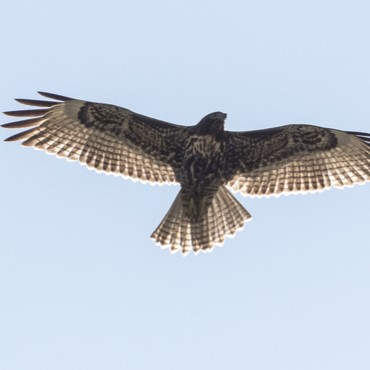
\includegraphics[width=0.49\linewidth,height=0.2\textheight]{animal_images/hawk_11} 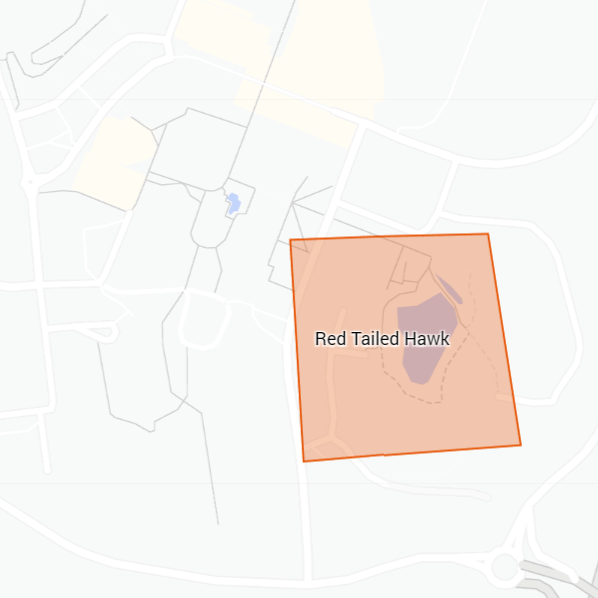
\includegraphics[width=0.49\linewidth,height=0.2\textheight]{animal_images/hawk_hotspot_11} 

}

\caption{Image of Red-tailed Hawk (*Buteo jamaicensis*). Image taken by [Bob Lalonde](https://www.inaturalist.org/photos/60514571), [CC BY-NC 4.0](https://creativecommons.org/licenses/by-nc/4.0/), via iNaturalist. Hot spot for Red tailed Hawk on campus.}\label{fig:unnamed-chunk-1}
\end{figure}

\hypertarget{great-horned-owl}{%
\section{Great Horned Owl}\label{great-horned-owl}}

This cool-looking bird may not give you sage advice like in Winnie the Pooh, but it is a nice encounter nonetheless! The Great Horned Owl (\emph{Bubo virginianus}) is believed to have migrated to North America from Eurasia back when there was a land bridge connecting what is now Alaska and Russia; they often share the same habitat and prey as the Red-Tailed Hawk, so if you see one, then you'll probably encounter the other. While the owl is cool, it can be a bit creepy when you hear it hooting around you when walking Pine Trail after a night lab\ldots{}

\begin{figure}

{\centering 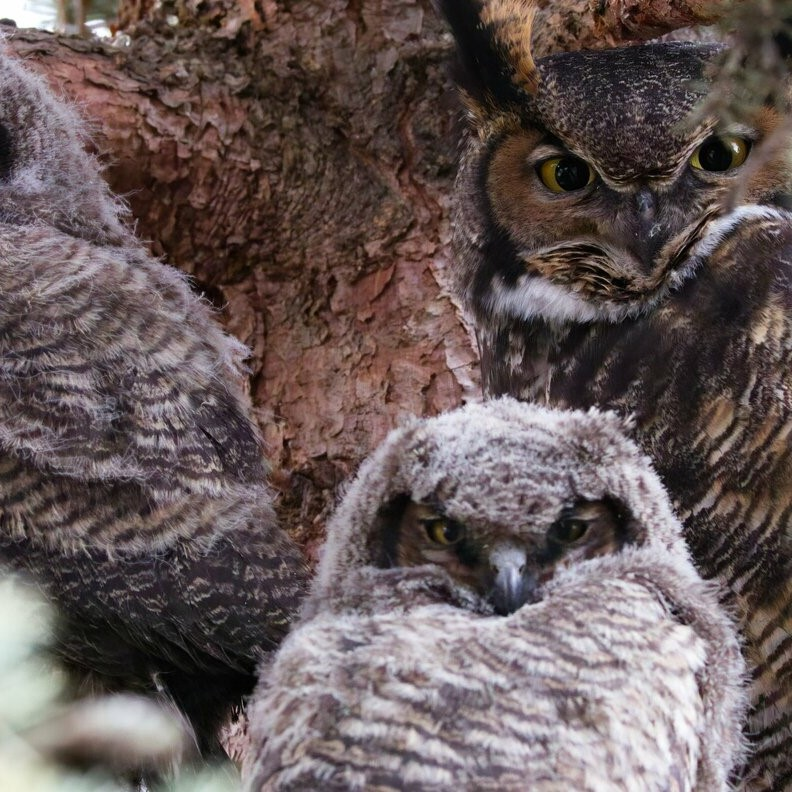
\includegraphics[width=0.49\linewidth,height=0.2\textheight]{animal_images/owl_11} 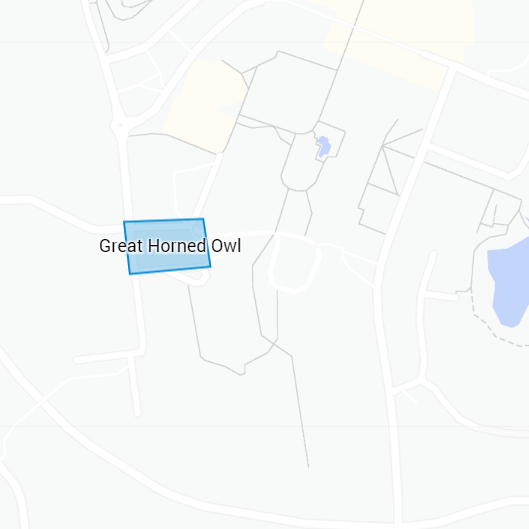
\includegraphics[width=0.49\linewidth,height=0.2\textheight]{animal_images/owl_hotspot_11} 

}

\caption{Image of Great Horned Owl (*Bubo virginianus*). Image taken by [Bob Lalonde](https://www.inaturalist.org/photos/260429890), [CC BY-NC 4.0](https://creativecommons.org/licenses/by-nc/4.0/), via iNaturalist. Hot spot for Great Horned Owl on campus.}\label{fig:unnamed-chunk-2}
\end{figure}

\hypertarget{northern-pacific-tree-frog}{%
\section{Northern Pacific Tree Frog}\label{northern-pacific-tree-frog}}

Say hello to the Northern Pacific Tree Frog (\emph{Pseudacris regilla}), a charming and slimy amphibian that is native to the Pacific Northwest. Found throughout western North America, including the forests and wetlands of Canada, this little green frog is known for its distinctive ribbiting call that can be heard echoing through the woods on warm summer nights. Despite its small size, the Northern Pacific Tree Frog is a mighty survivor, capable of hibernating through long, cold Canadian winters and thriving in a variety of aquatic and terrestrial habitats. These frogs are also an important indicator of environmental health, with declines in their populations signaling potential problems in wetland ecosystems. So if you're lucky enough to spot a Northern Pacific Tree Frog on your next stroll on campus, take a moment to appreciate this remarkable little creature and the important role it plays in the country's natural landscape!

\begin{figure}

{\centering 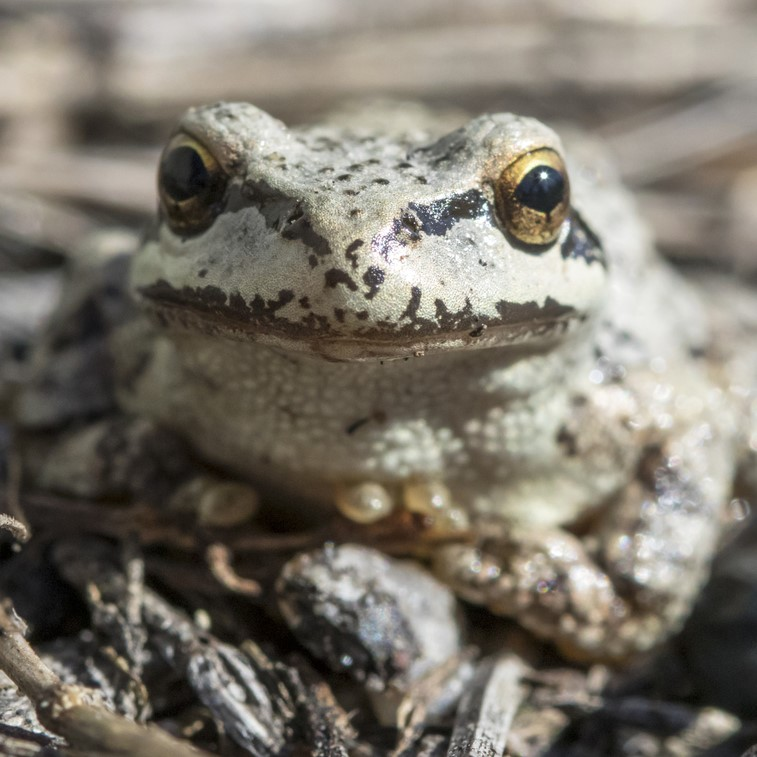
\includegraphics[width=0.49\linewidth,height=0.2\textheight]{animal_images/forg_11} 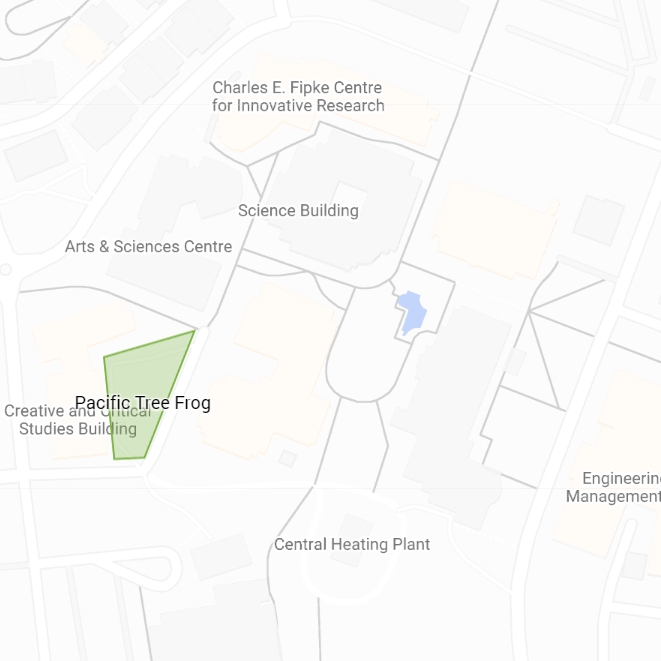
\includegraphics[width=0.49\linewidth,height=0.2\textheight]{animal_images/forg_hotspot_11} 

}

\caption{Image of Northern Pacific Tree Frog (*Pseudacris regilla*). Image taken by [Bob Lalonde](https://www.inaturalist.org/photos/60514377), [CC BY-NC 4.0](https://creativecommons.org/licenses/by-nc/4.0/), via iNaturalist. Hot spot for Northern Pacific Tree Frog on campus.}\label{fig:unnamed-chunk-3}
\end{figure}

\hypertarget{painted-turtle}{%
\section{Painted Turtle}\label{painted-turtle}}

Introducing the Western Painted Turtle (\emph{Chrysemys picta} ssp. \emph{bellii}), a colorful and cute reptile that is native to Canada and found in many of the country's freshwater habitats. These turtles are true works of art, with intricate patterns and bright colors that resemble those of a painting. They are also fascinating creatures, capable of spending long periods of time underwater and surviving in environments that are inhospitable to many other animals. However, despite their resilience, Western Painted Turtles face many threats, including habitat loss, climate change, and pollution. This has led to declines in their populations in some parts of Canada, making conservation efforts more important than ever. So if you're lucky enough to spot a Western Painted Turtle around EME, cherish the sight because they are at risk!

\begin{figure}

{\centering 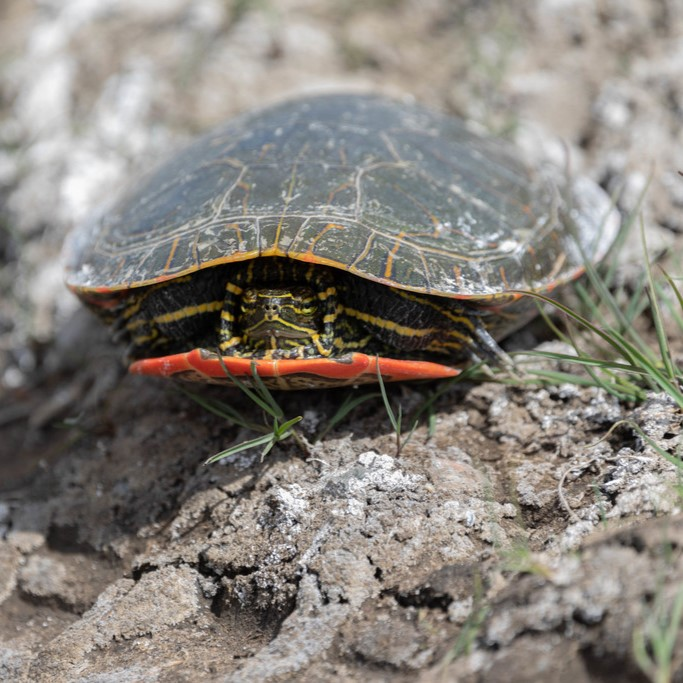
\includegraphics[width=0.49\linewidth,height=0.2\textheight]{animal_images/turt_11} 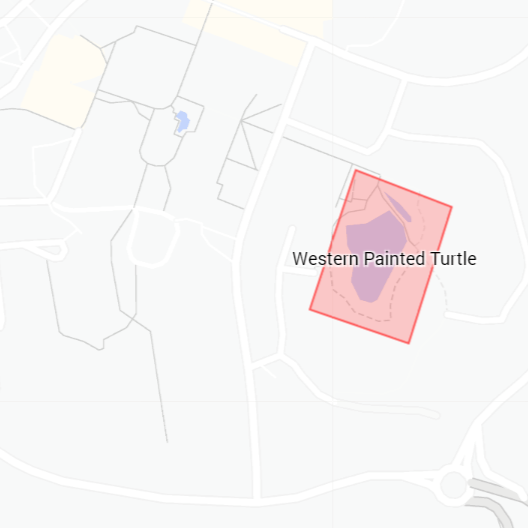
\includegraphics[width=0.49\linewidth,height=0.2\textheight]{animal_images/turt_hotspot_11} 

}

\caption{Image of Western Painted Turtle (*Chrysemys picta* ssp. *bellii*). Image taken by [Kalvin Chan](https://www.inaturalist.org/photos/123339228), [CC BY-NC 4.0](https://creativecommons.org/licenses/by/4.0/), via iNaturalist. Hot spot for Western Painted Turtle on campus.}\label{fig:unnamed-chunk-4}
\end{figure}

\hypertarget{mule-deer}{%
\section{Mule Deer}\label{mule-deer}}

Meet the Mule Deer (\emph{Odocoileus hemionus}), a striking and iconic species of deer that roams throughout the forests and mountains of Canada. Known for their large ears that resemble those of a mule, these deer are a common sight for Canadians who enjoy hiking and camping in the great outdoors. Despite their size and strength, Mule Deer are graceful creatures, able to bound over fallen logs and navigate rocky terrain with ease. They are also an important part of the country's hunting traditions, with regulated hunting seasons in many provinces helping to manage their populations. However, with growing concerns about habitat loss and climate change, the future of Mule Deer in Canada remains uncertain.

\begin{figure}

{\centering 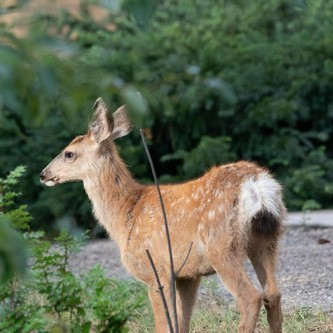
\includegraphics[width=0.49\linewidth,height=0.2\textheight]{animal_images/deer_11} 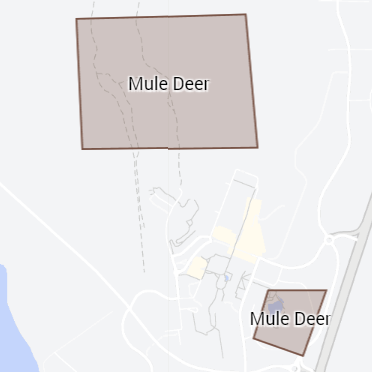
\includegraphics[width=0.49\linewidth,height=0.2\textheight]{animal_images/deer_hotspot_11} 

}

\caption{Image of Mule Deer (*Odocoileus hemionus*). Image taken by [Kalvin Chan](https://www.inaturalist.org/photos/224918782), [CC BY-NC 4.0](https://creativecommons.org/licenses/by/4.0/), via iNaturalist. Hot spot for Mule Deer on campus.}\label{fig:unnamed-chunk-5}
\end{figure}

\hypertarget{location}{%
\section{Location}\label{location}}

\hypertarget{insects-invertebrates}{%
\chapter{Insects (Invertebrates)}\label{insects-invertebrates}}

\hypertarget{knapweed-root-weevil}{%
\section{Knapweed Root Weevil}\label{knapweed-root-weevil}}

The knapweed root weevil (\emph{Cyphocleonus Achates}) is a fascinating species of weevil that has captured the attention of ecologists and entomologists alike. This beetle has a unique ability to control invasive plant populations, specifically knapweeds. They are used in BC as a biocontrol agent; meaning that while they are an introduced species they are actually beneficial to the ecosystem since they consume and control populations of invasive knapweeds that can outcompete native species as well as taking up nutrients from the soil that can be used by livestock and crops.

\begin{figure}

{\centering 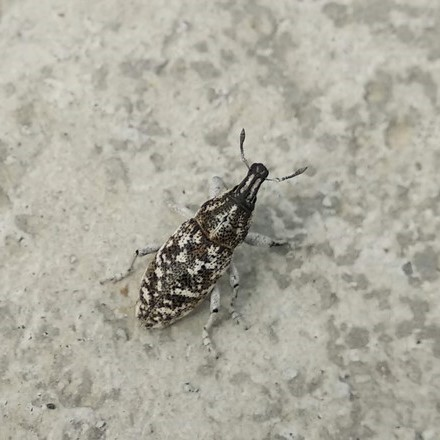
\includegraphics[width=0.49\linewidth,height=0.2\textheight]{insect_images/cyphocleonus_11} 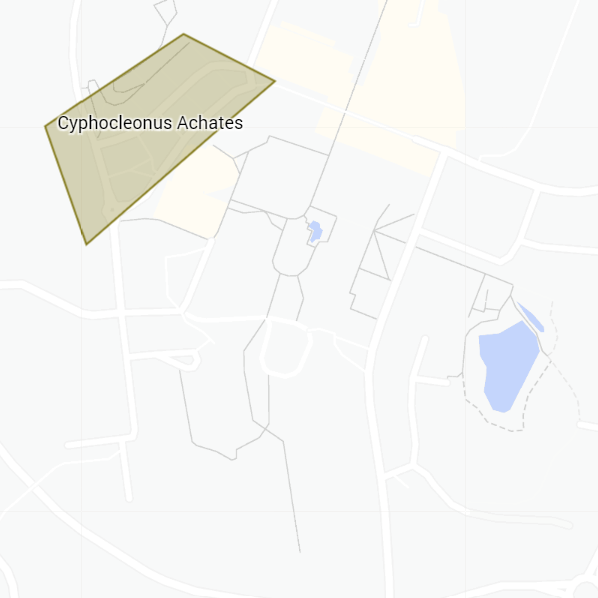
\includegraphics[width=0.49\linewidth,height=0.2\textheight]{insect_images/cyphocleonus_hotspot_11} 

}

\caption{Image of Knapweed Root Weevil (*Cyphocleonus Achates*). Image taken by [malreux](https://www.inaturalist.org/photos/24907280), [CC BY-NC 4.0](https://creativecommons.org/licenses/by-nc/4.0/), via iNaturalist. Hot spot for Cyphocleonus Achates on campus.}\label{fig:unnamed-chunk-6}
\end{figure}

\hypertarget{european-mantis}{%
\section{European Mantis}\label{european-mantis}}

While this member of the Mantidae family may seem delicate, it is anything but; from the female eating the male's head after mating to the fact that it is an invasive species to North America, the European mantis (\emph{Mantis religiosa}) is quite the pest. It was first introduced into North America in the 1900s as a biocontrol agent for gypsy moths but has since spread throughout the continent. This rapid spreading presents an ecological problem as the mantis predates native insects, disrupting local ecosystems.

\begin{figure}

{\centering 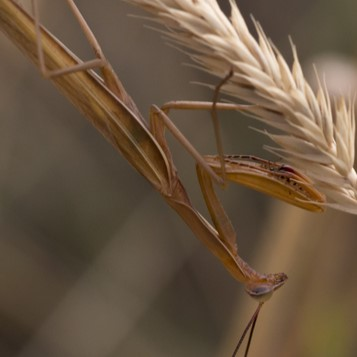
\includegraphics[width=0.49\linewidth,height=0.2\textheight]{insect_images/mantis_11} 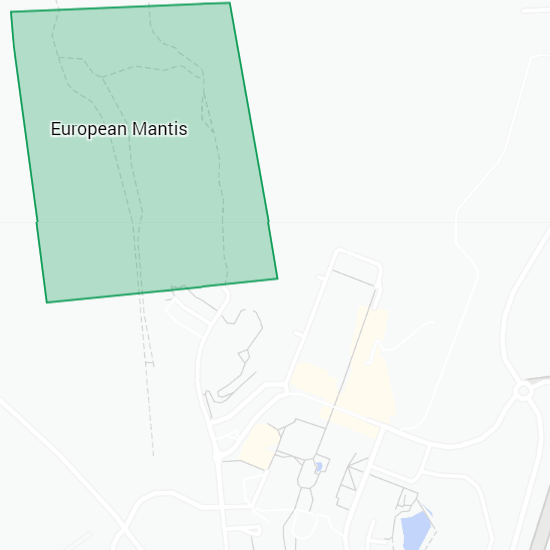
\includegraphics[width=0.49\linewidth,height=0.2\textheight]{insect_images/mantis_hotspot_11} 

}

\caption{Image of European Mantis (*Mantis religiosa*). Image taken by [Bob Lalonde](https://www.inaturalist.org/photos/60515212), [CC BY-NC 4.0](https://creativecommons.org/licenses/by-nc/4.0/), via iNaturalist. Hot spot for European Mantis on campus.}\label{fig:unnamed-chunk-7}
\end{figure}

\hypertarget{asian-lady-bug}{%
\section{Asian Lady Bug}\label{asian-lady-bug}}

The Asian ladybug (\emph{Harmonia axyridis}) is a captivating insect that has become a common sight in North America, including right here on campus. Originally introduced as a biological control for pests, such as aphids, this ladybug has since become well-established in many regions. These insects are quite different from the native ladybugs that most people are familiar with, as they can vary in coloration from orange to black and even have spots or stripes. They also have a peculiar habit of aggregating in large numbers during the fall, often seeking shelter in buildings and homes. While they may provide some benefits as predators of pests, their impact on native ladybug species and potential harm to agricultural crops is still being studied by ecologists.

\begin{figure}

{\centering 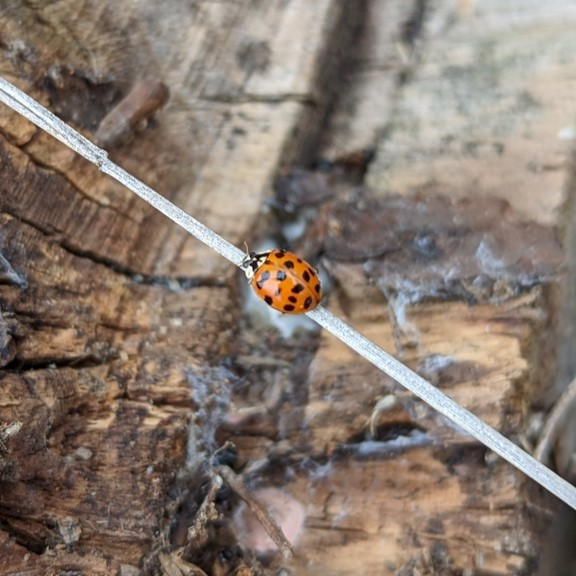
\includegraphics[width=0.49\linewidth,height=0.2\textheight]{insect_images/lady_11} 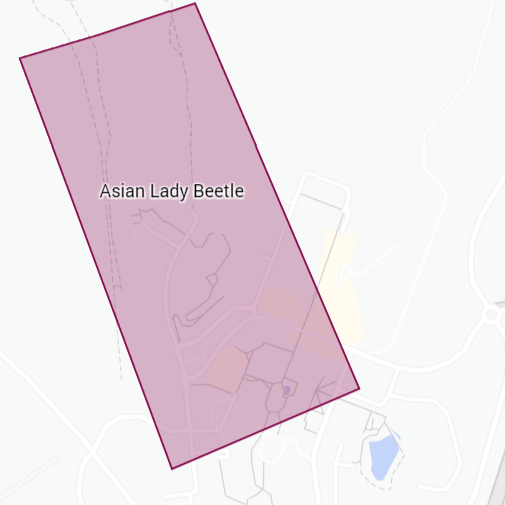
\includegraphics[width=0.49\linewidth,height=0.2\textheight]{insect_images/lady_hotspot_11} 

}

\caption{Image of Asian Lady Bug (*Harmonia axyridis*). Image taken by [kalvinchan](https://www.inaturalist.org/photos/230709327), [CC BY-NC 4.0](https://creativecommons.org/licenses/by/4.0/), via iNaturalist. Hot spot for Asian Lady Bug on campus.}\label{fig:unnamed-chunk-8}
\end{figure}

\hypertarget{leopard-slug}{%
\section{Leopard Slug}\label{leopard-slug}}

Welcome to the world of the Leopard Slug (\emph{Limax maximus}), a slimy and mesmerizing creature that is sure to capture your attention! This impressive gastropod, also known as Limax maximus, is a true wonder of the animal kingdom. With its distinctive leopard-like spots and elongated body that can stretch up to 8 inches long, it's hard to miss this incredible slug. Found in various parts of the world, including Europe, Asia, and North America, the Leopard Slug is not your average garden pest. Instead, it's a master of disguise, using its unique coloration and shape to blend seamlessly into its surroundings. So if you're ready to learn more about this slimy superstar, keep an eye out when your walking around campus next time it rains!

\begin{figure}

{\centering 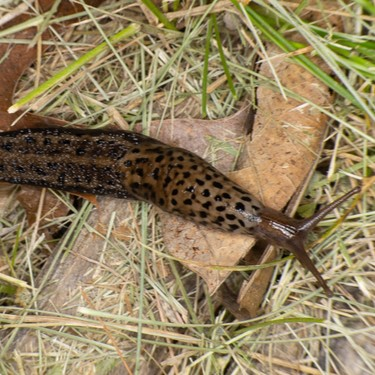
\includegraphics[width=0.49\linewidth,height=0.2\textheight]{insect_images/slug_11} 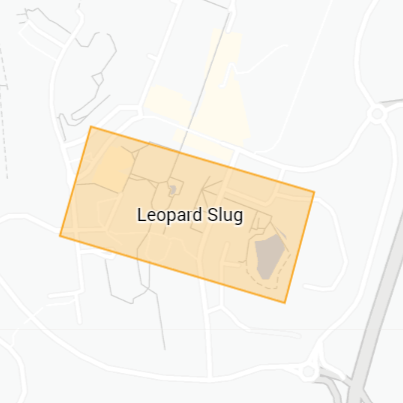
\includegraphics[width=0.49\linewidth,height=0.2\textheight]{insect_images/slug_hotspot_11} 

}

\caption{Image of Leopard Slug (*Limax maximus*). Image taken by [Jason Alexander](https://www.inaturalist.org/photos/80439924), [CC BY-NC 4.0](https://creativecommons.org/licenses/by-nc/4.0/), via iNaturalist. Hot spot for Leopard Slug on campus.}\label{fig:unnamed-chunk-9}
\end{figure}

\hypertarget{california-broad-necked-beetle}{%
\section{California Broad Necked Beetle}\label{california-broad-necked-beetle}}

The California broad-necked beetle (\emph{Coelocnemis dilaticollis}) is a stunning insect that is native to the western region of North America. This beetle is around 12-15mm in length and has a unique shape that sets it apart from other beetles. Its broad, flattened neck gives it an almost distinct hourglass shape and its metallic green coloration adds to its beauty. The California broad-necked beetle can usually be found on the flowers and foliage of oak trees, primarily in the late spring and early summer months. It serves as an important part of the ecosystem by pollinating and aiding in the decomposition process. Sightings have been spread all throughout campus even up on Old Pine Trail so watch your step!

\begin{figure}

{\centering 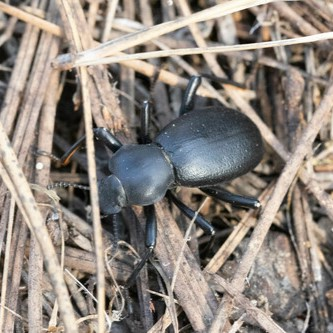
\includegraphics[width=0.49\linewidth,height=0.2\textheight]{insect_images/cali_beet_11} 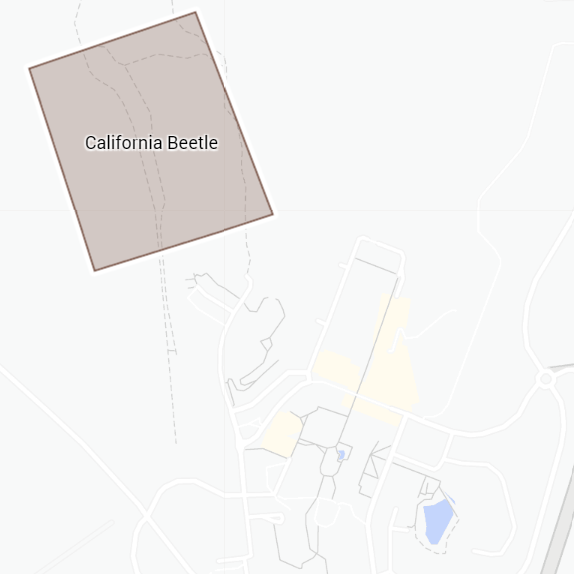
\includegraphics[width=0.49\linewidth,height=0.2\textheight]{insect_images/cali_beet_hotspot_11} 

}

\caption{Image of California broad-necked beetle (*Coelocnemis dilaticollis*). Image taken by [kalvinchan](https://www.inaturalist.org/photos/233670239), [CC BY-NC 4.0](https://creativecommons.org/licenses/by/4.0/), via iNaturalist. Hot spot for California broad-necked beetle on campus.}\label{fig:unnamed-chunk-10}
\end{figure}

\hypertarget{location-1}{%
\section{Location}\label{location-1}}

\hypertarget{plantsfungi}{%
\chapter{Plants/Fungi}\label{plantsfungi}}

\hypertarget{horse-chestnut}{%
\section{Horse Chestnut}\label{horse-chestnut}}

Horse chestnut (\emph{Aesculus hippocastanum}) is a large tree that can reach up to 100 feet tall. It is a native species of the Balkans and was introduced to other parts of Europe and North America in the 16th century. Horse chestnut provides food and shelter for a variety of animals, including bees, birds, squirrels, and deer. For the microbio majors out there, it can be used to extract aesculin, a glucoside that is hydrolyzed by Enterococci making it useful for detection assays! Although the fruits of this tree look similar to chestnuts, they should not be eaten! The fruits contain large amounts of saponins which are toxic to humans\ldots{}

\begin{figure}

{\centering 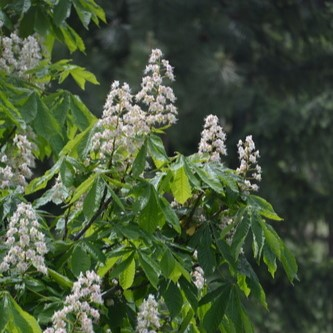
\includegraphics[width=0.49\linewidth,height=0.2\textheight]{plant_images/horse_c_11} 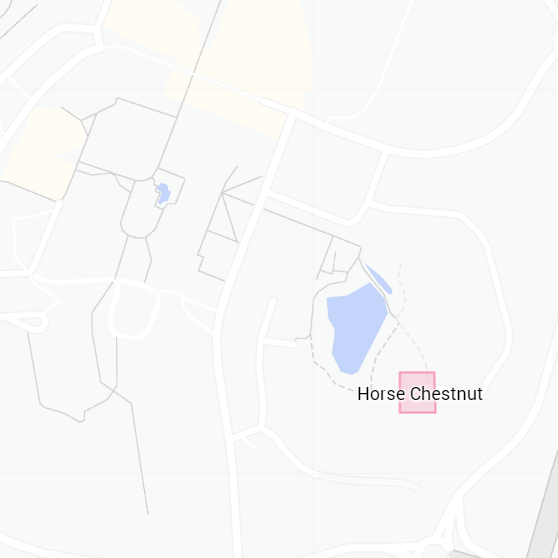
\includegraphics[width=0.49\linewidth,height=0.2\textheight]{plant_images/horse_c_hotspot_11} 

}

\caption{Image of Horse Chestnut (*Aesculus hippocastanum*). Image taken by [lesfreck](https://www.inaturalist.org/photos/201399267), [CC BY-NC 4.0](https://creativecommons.org/licenses/by-nc/4.0/), via iNaturalist. Hot spot for Horse-Chestnut on campus.}\label{fig:unnamed-chunk-11}
\end{figure}

\hypertarget{bonnets}{%
\section{Bonnets}\label{bonnets}}

Bonnets (Genus \emph{Mycena}) are marvels of nature! These beautiful, bulbous fungi are a vital part of our local ecological web, providing nourishment and shelter for a wide array of creatures. Some species of bonnets are also known to have medicinal properties, making them valuable not just for their ecological role. The edibility of these mushrooms varies across species, so maybe don't use them for your ravioli. Take a moment to appreciate the intricate beauty of bonnets as you walk along the EME pond or Old Pine Trail, and you'll see just how cool and interesting these plants are.

\begin{figure}

{\centering 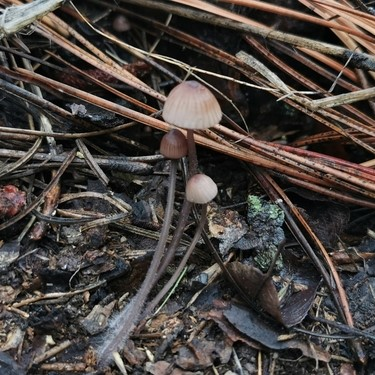
\includegraphics[width=0.49\linewidth,height=0.2\textheight]{plant_images/bonnets_11} 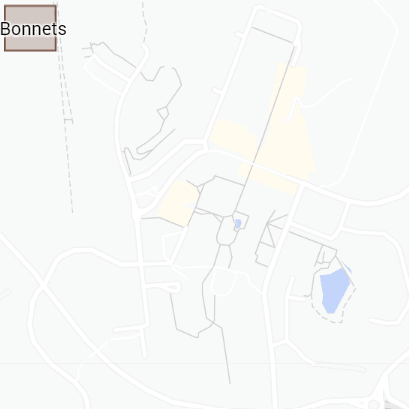
\includegraphics[width=0.49\linewidth,height=0.2\textheight]{plant_images/bonnets_hotspot_11} 

}

\caption{Image of Bonnets (Genus *Mycena*). Image taken by [kalvinchan](https://www.inaturalist.org/photos/170911702), [CC BY-NC 4.0](https://creativecommons.org/licenses/by-nc/4.0/), via iNaturalist. Hot spot for bonnets on campus.}\label{fig:unnamed-chunk-12}
\end{figure}

\hypertarget{silvery-cinquefoil}{%
\section{Silvery Cinquefoil}\label{silvery-cinquefoil}}

Silvery cinquefoil (\emph{Potentilla argentea}) is a striking silver-leaved plant that looks like it's out of a fairytale. This subalpine plant has delicate five-petaled yellow flowers that bloom in dense clusters on long stems that reach about 20 cm tall. The angled, five-toothed leaves are covered with fine silver hairs on the bottom, creating a unique shimmering effect that catches the eye. Silvery cinquefoil is an invasive species that originates from Eurasia. It thrives in harsh, rocky environments. Despite its alluring appearance, silvery cinquefoil is considered a pest in BC.

\begin{figure}

{\centering 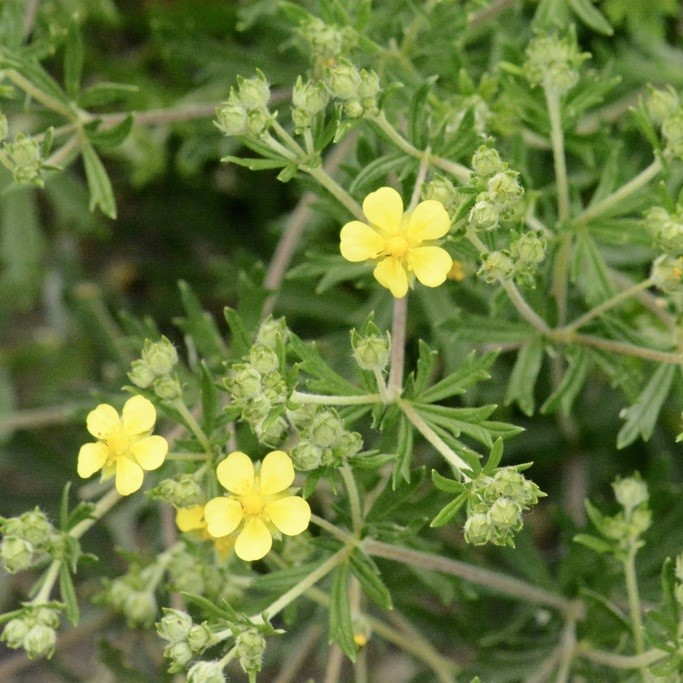
\includegraphics[width=0.49\linewidth,height=0.2\textheight]{plant_images/silvery_cinq_11} 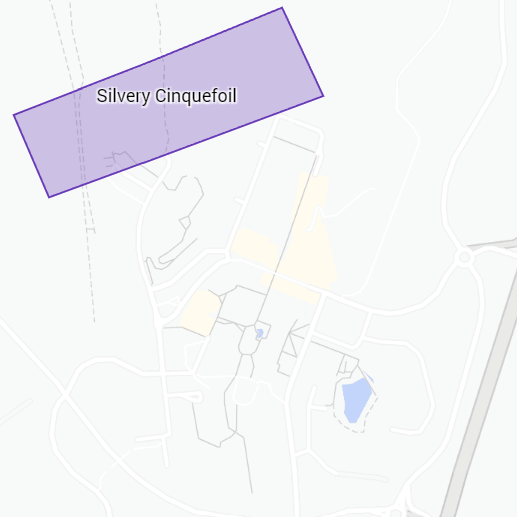
\includegraphics[width=0.49\linewidth,height=0.2\textheight]{plant_images/silveryconquefoil_hotspot_11} 

}

\caption{Image of Silvery Cinquefoil (*Potentilla argentea*). Image taken by [lesfreck](https://www.inaturalist.org/photos/198692554), [CC BY-NC 4.0](https://creativecommons.org/licenses/by-nc/4.0/), via iNaturalist. Hot spot for Silvery Cinquefoil on campus.}\label{fig:unnamed-chunk-13}
\end{figure}

\hypertarget{bittersweet-nightshade}{%
\section{Bittersweet Nightshade}\label{bittersweet-nightshade}}

Bittersweet nightshade (\emph{Solanum dulcamara}) is a fascinating perennial plant that belongs to the nightshade family, which includes many common vegetables such as tomatoes, aubergines, potatoes, and bell peppers! This plant boasts small, star-shaped purple or white flowers that give way to shiny, red berries. Beware, though, as their bright and juicy berries can be tempting, their hollow stem and leaves contain a bitter toxin that can cause nausea, vomiting, and hallucinations. Native to Asia and Europe, bittersweet nightshade has a long history of traditional medicinal use, but it is also a standout in the world of ecology. Due to its aggressive nature and ability to adapt to a wide range of habitats, bittersweet nightshade is classified as an invasive species in many regions including the Thompson-Okanagan. So while its beauty and intrigue may be captivating, it's important to remember that bittersweet nightshade is a complex and extremely dangerous plant that serves as a reminder of the delicate balance of our natural world. Be sure to be on the lookout next time you take a study break around the pound behind EME!

\begin{figure}

{\centering 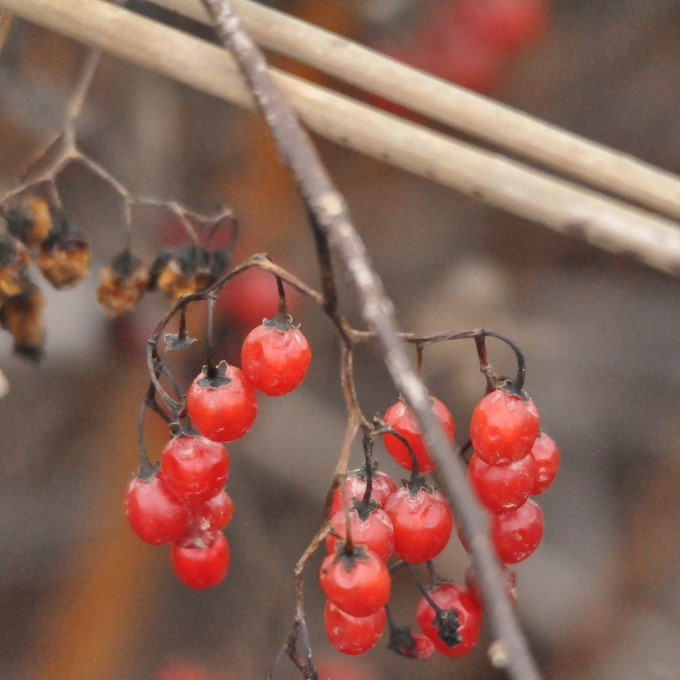
\includegraphics[width=0.31\linewidth,height=0.2\textheight]{plant_images/bitter_night_red_11} 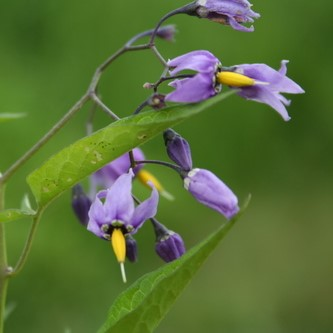
\includegraphics[width=0.31\linewidth,height=0.2\textheight]{plant_images/bitter_night_purp_11} 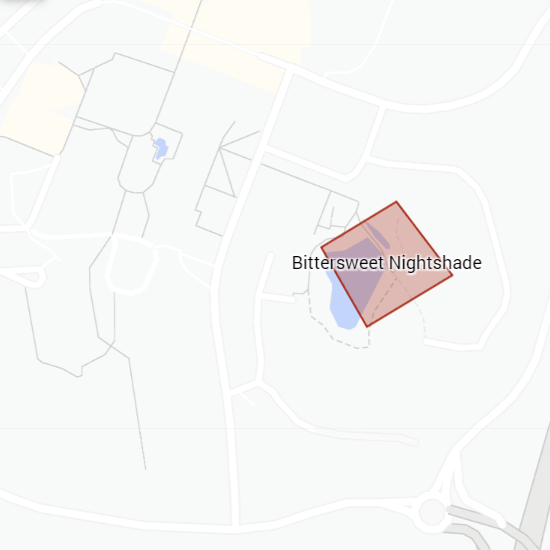
\includegraphics[width=0.31\linewidth,height=0.2\textheight]{plant_images/bitter_night_hotspot_11} 

}

\caption{Images of Bittersweet Nightshade (*Solanum dulcamara*). Left most image taken by [lesfreck](https://www.inaturalist.org/photos/61694401), [CC BY-NC 4.0](https://creativecommons.org/licenses/by-nc/4.0/), via iNaturalist. Middle image taken by [Alexander Baransky](https://www.inaturalist.org/photos/70860715), CC BY-NC 4.0, via iNaturalist. Hot spot for Bittersweet Nightshade on campus.}\label{fig:unnamed-chunk-14}
\end{figure}

\hypertarget{wolf-lichen}{%
\section{Wolf Lichen}\label{wolf-lichen}}

Wolf lichen (\emph{Letharia vulpina}) is a lichen, which means that it is actually two organisms! Lichens are composite organisms made from symbiotic partnerships between fungi and algae. Wolf Lichen is yellow-green in colour, shrubby and highly branched. It most often grows on the bark of living and dead conifers. The pigment that gives wolf lichen its yellow colour (vulpinic acid) is slightly toxic to mammals. The toxic pigment was used historically to poison wolves, which is the inspiration for the name wolf lichen.

\begin{figure}

{\centering 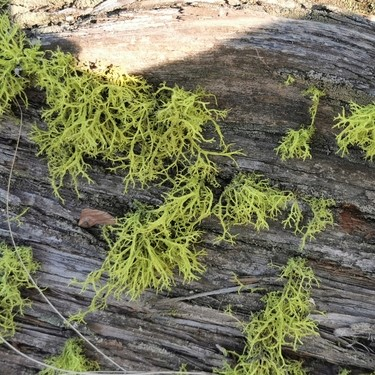
\includegraphics[width=0.49\linewidth,height=0.2\textheight]{plant_images/wolf_inat_11} 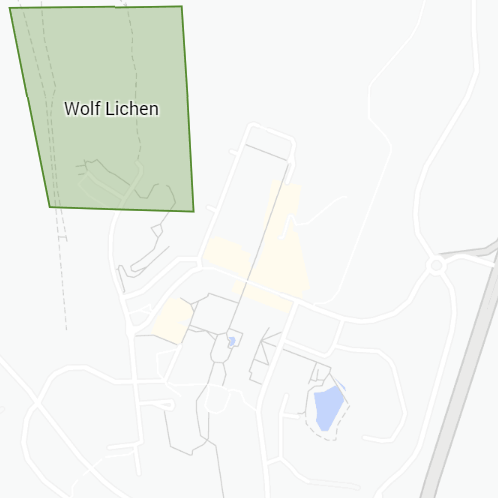
\includegraphics[width=0.49\linewidth,height=0.2\textheight]{plant_images/wolflichen_hotspot_11} 

}

\caption{Image of Wolf Lichen (*Letharia vulpina*). Image taken by [kalvinchan](https://www.inaturalist.org/photos/179070916), [CC BY-NC 4.0](https://creativecommons.org/licenses/by-nc/4.0/), via iNaturalist. Hot spot for Wolf Lichen on campus.}\label{fig:unnamed-chunk-15}
\end{figure}

\hypertarget{location-2}{%
\section{Location}\label{location-2}}

\hypertarget{acknowledgements}{%
\chapter{Acknowledgements}\label{acknowledgements}}

Thank you to iNaturalist and its contributors for the data needed for this project:

\begin{center}
\includegraphics[width=0.99\linewidth,height=0.2\textheight]{partner_images/inat} \end{center}

Special thanks to our campus partners:

\begin{center}
\includegraphics[width=0.99\linewidth,height=0.2\textheight]{partner_images/wild-ccu} \end{center}

\begin{center}
\includegraphics[width=0.49\linewidth,height=0.2\textheight]{partner_images/micbio} 
\includegraphics[width=0.49\linewidth,height=0.2\textheight]{partner_images/igem} \end{center}

  \bibliography{book.bib,packages.bib}

\end{document}
